% -----------------------------------------------------------------------
% outputs.tex: Section detailing the different forms of text- and
%              plot-based output.
% -----------------------------------------------------------------------
% Copyright (C) 2006, Matthew Whiting, ATNF
%
% This program is free software; you can redistribute it and/or modify it
% under the terms of the GNU General Public License as published by the
% Free Software Foundation; either version 2 of the License, or (at your
% option) any later version.
%
% Duchamp is distributed in the hope that it will be useful, but WITHOUT
% ANY WARRANTY; without even the implied warranty of MERCHANTABILITY or
% FITNESS FOR A PARTICULAR PURPOSE.  See the GNU General Public License
% for more details.
%
% You should have received a copy of the GNU General Public License
% along with Duchamp; if not, write to the Free Software Foundation,
% Inc., 59 Temple Place, Suite 330, Boston, MA 02111-1307, USA
%
% Correspondence concerning Duchamp may be directed to:
%    Internet email: Matthew.Whiting [at] atnf.csiro.au
%    Postal address: Dr. Matthew Whiting
%                    Australia Telescope National Facility, CSIRO
%                    PO Box 76
%                    Epping NSW 1710
%                    AUSTRALIA
% -----------------------------------------------------------------------
\secA{Outputs}
\label{sec-output}

\secB{During execution}

\duchamp provides the user with feedback whilst it is running, to
keep the user informed on the progress of the analysis. Most of this
consists of self-explanatory messages about the particular stage the
program is up to. The relevant parameters are printed to the screen at
the start (once the file has been successfully read in), so the user
is able to make a quick check that the setup is correct (see
Appendix~{app-input} for an example).

If the cube is being trimmed (\S\ref{sec-modify}), the resulting
dimensions are printed to indicate how much has been trimmed. If a
reconstruction is being done, a continually updating message shows
either the current iteration and scale, compared to the maximum scale
(when \texttt{reconDim = 3}), or a progress bar showing the amount of
the cube that has been reconstructed (for smaller values of
\texttt{reconDim}).

During the searching algorithms, the progress through the search is
shown. When completed, the number of objects found is reported (this
is the total number found, before any merging is done).

In the merging process (where multiple detections of the same object
are combined -- see \S\ref{sec-merger}), two stages of output
occur. The first is when each object in the list is compared with all
others. The output shows two numbers: the first being how far through
the list the current object is, and the second being the length of the
list. As the algorithm proceeds, the first number should increase and
the second should decrease (as objects are combined). When the numbers
meet, the whole list has been compared. If the objects are being
grown, a similar output is shown, indicating the progress through the
list. In the rejection stage, in which objects not meeting the minimum
pixels/channels requirements are removed, the total number of objects
remaining in the list is shown, which should steadily decrease with
each rejection until all have been examined. Note that these steps can
be very quick for small numbers of detections.

Since this continual printing to screen has some overhead of time and
CPU involved, the user can elect to not print this information by
setting the parameter \texttt{verbose = false}. In this case, the user
is still informed as to the steps being undertaken, but the details of
the progress are not shown.

There may also be Warning or Error messages printed to screen. The
Warning messages occur when something happens that is unexpected (for
instance, a desired keyword is not present in the FITS header), but
not detrimental to the execution. An Error message is something more
serious, and indicates some part of the program was not able to
complete its task. The message will also indicate which function or
subroutine generated it -- this is primarily a tool for debugging, but
can be useful in determining what went wrong.

\secB{Text-based output files}

\secC{Table of results}
\label{sec-results}

Finally, we get to the results -- the reason for running \duchamp in
the first place. Once the detection list is finalised, it is sorted
according to the value of the \texttt{sortingParam}. This can take the
value ``x-value'', ``y-value'', ``z-value'', ``ra'', ``dec'', ``vel'',
``w50'', ``iflux'' (for integrated flux), or ``pflux'' (for peak
flux), or ``snr''. The default value is ``vel''. If no good WCS
exists, the mean pixel position equivalent is used (``ra'' is replaced
by ``x-value'', ``dec'' by ``y-value'', ``vel'' and ``w50'' by
``z-value''). The results are then printed to the screen and to the
output file, given by the \texttt{OutFile} parameter.

The output consists of two sections. First, a list of the parameters
are printed to the output file, for future reference. Next, the
detection threshold that was used is given, so comparison can be made
with other searches. The statistics estimating the noise parameters
are given (see \S\ref{sec-stats}). Thirdly, the number of detections
are reported.

All this information, known as the ``header'', can either be written
to the start of the output file (denoted by the parameter
\texttt{OutFile}), or written to a separate file from the list of
detections. This second option is activated by the parameter
\texttt{flagSeparateHeader}, and the information is written to the
file given by \texttt{HeaderFile}.

The most interesting part, however, is the list of detected
objects. This list, an example of which can be seen in
Appendix~\ref{app-output}, contains the following columns (note that
the title of the columns depending on WCS information will depend on
the details of the WCS projection: they are shown below for the
Equatorial and Galactic projection cases).

\begin{Lentry}
\item[{Obj\#}] The ID number of the detection (simply the
  sequential count for the list, which is ordered by increasing
  velocity, or channel number, if the WCS is not good enough to find
  the velocity).
\item[{Name}] The ``IAU''-format name of the detection (derived from the
  WCS position -- see below for a description of the format).
\item[{X,Y,Z}] The ``centre'' pixel position, determined by the input
  parameter \texttt{pixelCentre}.
\item[{RA/GLON}] The Right Ascension or Galactic Longitude of the centre
  of the object.
\item[{DEC/GLAT}] The Declination or Galactic Latitude of the centre of
  the object.
\item[{VEL}] The mean velocity of the object [units given by the
  \texttt{spectralUnits} parameter].
\item[{w\_RA/w\_GLON}] The width of the object in Right Ascension or
  Galactic Longitude (depending on FITS coordinates) [arcmin].
\item[{w\_DEC/w\_GLAT}] The width of the object in Declination Galactic
  Latitude [arcmin].
\item[{w\_50}] The velocity width of the detection at 50\% of the peak
  flux (the measured full-width at half-maximum, FWHM), in velocity
  units [see note below].
\item[{F\_int}] The integrated flux over the object, in the units of
  flux times velocity, corrected for the beam if necessary.
\item[{F\_peak}] The peak flux over the object, in the units of flux.
\item[{S/Nmax}] The signal-to-noise ratio at the peak pixel.
\item[{X1, X2}] The minimum and maximum X-pixel coordinates.
\item[{Y1, Y2}] The minimum and maximum Y-pixel coordinates.
\item[{Z1, Z2}] The minimum and maximum Z-pixel coordinates.
\item[{Npix}] The number of voxels (\ie distinct $(x,y,z)$ coordinates)
  in the detection.
\item[{Flag}] Whether the detection has any warning flags (see below).
\end{Lentry}

These parameters are written to the screen during execution. There are
alternative ways of calculating the total flux, the position and
velocity width, however, and so additional parameters are written to
the output file:
\begin{Lentry}
\item[{w\_20}] The velocity width of the detection at 20\% of the peak
  flux, in velocity units [see note below].
\item[{w\_VEL}] The full velocity width of the detection (max channel
  $-$ min channel, in velocity units).
\item[{F\_tot}] The sum of the flux values of all detected voxels.
\item[{X\_av, Y\_av, Z\_av}] The average pixel value in each
  axis direction \ie X\_av is the average of the $x$-values of all
  pixels in the detection.
\item[{X\_cent, Y\_cent, Z\_cent}] The centroid position, being
  the flux-weighted average of the pixels.
\item[{X\_peak, Y\_peak, Z\_peak}] The location of the pixel
  containing the peak flux value.
\end{Lentry}
The velocity width of the detection is calculated at 50\% and 20\% of
the peak flux, as well as the full detected width (if the detection
threshold is greater than 20\% or 50\% of the peak, then these values
will be the same as \texttt{w\_VEL}. The type of position value given
in the \texttt{X, Y, Z} columns in the screen output is determined by
the \texttt{pixelCentre} parameter. All three alternatives are shown
in the output file.

The user can specify the precision used to display the flux, velocity
and S/Nmax values, by using the input parameters \texttt{precFlux},
\texttt{precVel} and \texttt{precSNR} respectively. These values apply
to the tables written to the screen and to the output file, as well as
for the VOTable (see below).

The \texttt{Name} is derived from the WCS position. For instance, a
source that is centred on the RA,Dec position 12$^h$53$^m$45$^s$,
-36$^\circ$24$'$12$''$ will be given the name J125345$-$362412, if the
epoch is J2000, or the name B125345$-$362412 if it is B1950. An
alternative form is used for Galactic coordinates: a source centred on
the position ($l$,$b$) = (323.1245, 5.4567) will be called
G323.124$+$05.457. If the WCS is not valid (\ie is not present or does
not have all the necessary information), the \texttt{Name, RA, DEC,
VEL} and related columns are not printed, but the pixel coordinates
are still provided.

The velocity units can be specified by the user, using the parameter
\texttt{spectralUnits} (enter it as a single string with no
spaces). The default value is km/s, which should be suitable for most
users. These units are also used to give the units of integrated
flux. Note that if there is no rest frequency specified in the FITS
header, the \duchamp output will instead default to using Frequency,
with units of MHz.

If the WCS is absent or not sufficiently specified, then all columns
from \texttt{RA/GLON} to \texttt{w\_VEL} will be left blank. Also,
\texttt{F\_int} will be replaced with the more simple \texttt{F\_tot}.

The \texttt{Flag} column contains any warning flags, such as:
\begin{itemize}
\item \textbf{E} -- The detection is next to the spatial edge of the image,
meaning either the limit of the pixels, or the limit of the non-BLANK
pixel region.
\item \textbf{S} -- The detection lies at the edge of the spectral region. 
\item \textbf{N} -- The total flux, summed over all the (non-BLANK)
pixels in the smallest box that completely encloses the detection, is
negative. Note that this sum is likely to include non-detected
pixels. It is of use in pointing out detections that lie next to
strongly negative pixels, such as might arise due to interference --
the detected pixels might then also be due to the interference, so
caution is advised.
\end{itemize}
In the absence of any of these flags, a \textbf{-} will be recorded in
this column.

\secC{Other results lists}

Three additional results files can also be requested. One option is a
VOTable-format XML file, containing just the RA, Dec, Velocity and the
corresponding widths of the detections, as well as the fluxes. The
user should set \texttt{flagVOT = true}, and put the desired filename
in the parameter \texttt{votFile} -- note that the default is for it
not to be produced. This file should be compatible with all Virtual
Observatory tools (such as Aladin%
\footnote{%Aladin can be found on the web at
\href{http://aladin.u-strasbg.fr/}{http://aladin.u-strasbg.fr/}}
or TOPCAT\footnote{%Tool for OPerations on Catalogues And Tables:
\href{http://www.star.bristol.ac.uk/~mbt/topcat/}%
{http://www.star.bristol.ac.uk/~mbt/topcat/}}). 

A second option is an annotation file for use with the Karma toolkit
of visualisation tools (in particular, with \texttt{kvis}). There are
two options on how objects are represented, governed by the
\texttt{annotationType} parameter. Setting this to \texttt{borders}
results in a border being drawn around the spatial pixels of the
object, in a manner similar to that seen in Fig.~\ref{fig-spect}. Note
that Karma/\texttt{kvis} does not always do this perfectly, so the
lines may not be directly lined up with pixel borders. The other
option is \texttt{annotationType = circles}. This will draw a circle
at the position of each detection, scaled by the spatial size of the
detection, and number it according to the Obj\# given above. To make
use of this option, the user should set \texttt{flagKarma = true}, and
put the desired filename in the parameter \texttt{karmaFile} -- again,
the default is for it not to be produced.

The final optional results file produced is a simple text file that
contains the spectra for each detected object. The format of the file
is as follows: the first column has the spectral coordinate, over the
full range of values; the remaining columns represent the flux values
for each object at the corresponding spectral position. The flux value
used is the same as that plotted in the spectral plot detailed below,
and governed by the \texttt{spectralMethod} parameter. An example of
what a spectral text file might look like is given below:

\begin{quote}
  {\footnotesize
    \begin{tabular}{lllll}
      1405.00219727  &0.01323344  &0.23648241  &0.04202826  &-0.00506790  \\
      1405.06469727  &0.01302835  &0.27393046  &0.04686056  &-0.00471084  \\
      1405.12719727  &0.01583361  &0.27760920  &0.04114933  &-0.01168737  \\
      1405.18969727  &0.01271889  &0.31489247  &0.03307962  &-0.00300790  \\
      1405.25219727  &0.01597644  &0.30401203  &0.05356426  &-0.00551653  \\
      1405.31469727  &0.00773827  &0.30031312  &0.04074831  &-0.00570147  \\
      1405.37719727  &0.00738304  &0.27921870  &0.05272378  &-0.00504959  \\
      1405.43969727  &0.01353923  &0.26132512  &0.03667958  &-0.00151006  \\  
      1405.50219727  &0.01119724  &0.28987029  &0.03497849  &-0.00645589  \\  
      1405.56469727  &0.00813379  &0.29839963  &0.04711142  &0.00536576   \\  
      1405.62719727  &0.00774377  &0.26530230  &0.04620502  &0.00724631   \\  
      1405.68969727  &0.00576067  &0.23215000  &0.04995513  &0.00290841   \\ 
      1405.75219727  &0.00452834  &0.16484940  &0.04261605  &-0.00612812  \\  
      1405.81469727  &0.01406293  &0.15989439  &0.03817926  &-0.00758385  \\ 
      1405.87719727  &0.01116611  &0.11890682  &0.05499069  &-0.00626362  \\  
      1405.93969727  &0.00687582  &0.10620256  &0.04743370  &0.00055177   \\
      $\vdots$       &$\vdots$    &$\vdots$    &$\vdots$    &$\vdots$     \\
    \end{tabular}
  }
\end{quote}

In addition to these three files, a log file can also be produced. As
the program is running, it also (optionally) records the detections
made in each individual spectrum or channel (see \S\ref{sec-detection}
for details on this process). This is recorded in the file given by
the parameter \texttt{LogFile}. This file does not include the columns
\texttt{Name, RA, DEC, w\_RA, w\_DEC, VEL, w\_VEL}. This file is
designed primarily for diagnostic purposes: \eg to see if a given set
of pixels is detected in, say, one channel image, but does not survive
the merging process. The list of pixels (and their fluxes) in the
final detection list are also printed to this file, again for
diagnostic purposes. The file also records the execution time, as well
as the command-line statement used to run \duchamp. The creation of
this log file can be prevented by setting \texttt{flagLog = false}
(which is the default).

\secB{Graphical output}

\begin{figure}[t]
  \begin{center}
    \includegraphics[width=\textwidth]{example_spectrum}
  \end{center}
  \caption{\footnotesize An example of the spectral output. Note several
    of the features discussed in the text: the red lines indicating the
    reconstructed spectrum; the blue dashed lines indicating the
    spectral extent of the detection; the green hashed area indicating
    the Milky Way channels that are ignored by the searching algorithm;
    the blue border showing its spatial extent on the 0th moment map;
    and the 15~arcmin-long scale bar.}
  \label{fig-spect}
\end{figure}

\begin{figure}[!t]
  \begin{center}
    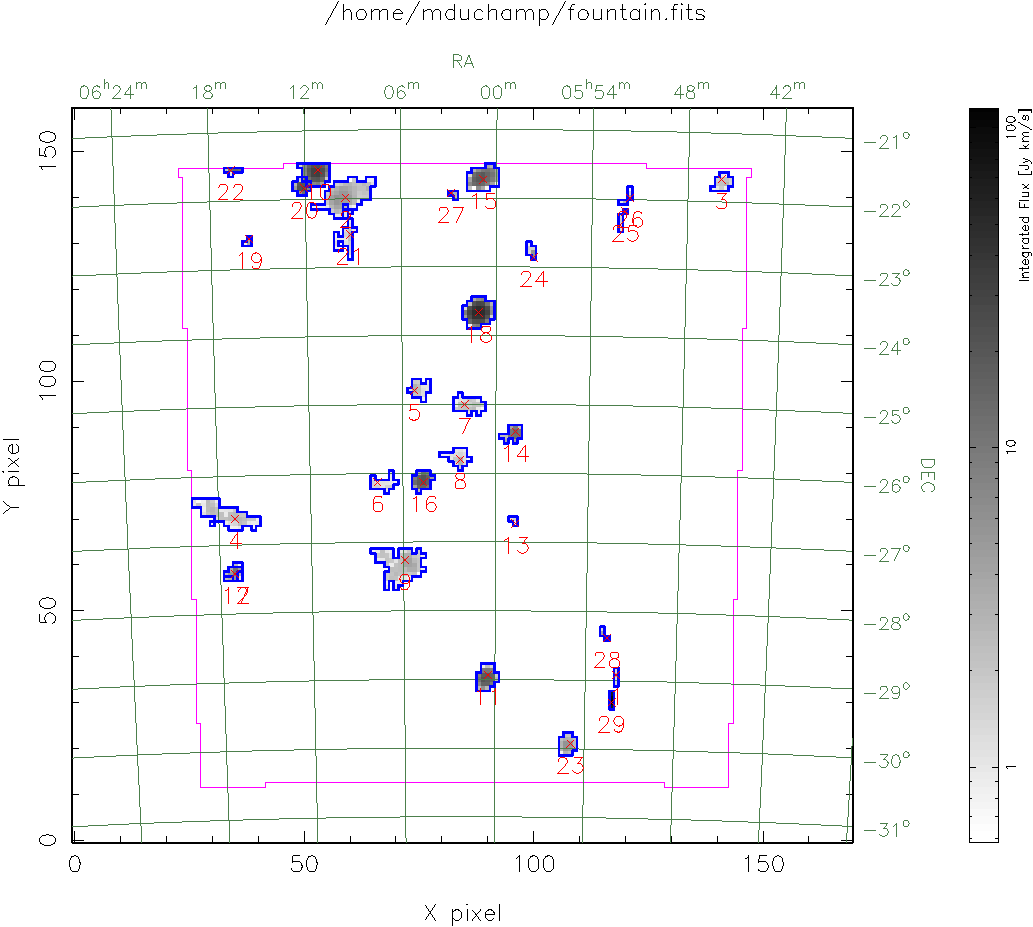
\includegraphics[width=\textwidth]{example_moment_map}
  \end{center}
  \caption{\footnotesize An example of the moment map created by
    \duchamp. The full extent of the cube is covered, and the 0th moment
    of each object is shown (integrated individually over all the
    detected channels). The purple line indicates the limit of the
    non-BLANK pixels.}
  \label{fig-moment}
\end{figure}

\secC{Mask image}
\label{sec-maskOut}

It is possible to create a FITS file containing a mask array. This
array is designed to indicate the location of detected objects. The
value of the detected pixels is determined by the
\texttt{flagMaskWithObjectNum} parameter: if \texttt{true}, the value
of the pixels is given by the corresponding object ID number; if
\texttt{false}, they take the value 1 for all objects. Pixels not in a
detected object have the value 0. To create this FITS file, set the
input parameter \texttt{flagOutputMask=true}. The file will be named
according to the \texttt{fileOutputMask} parameter, or, if this is not
given, \texttt{image.MASK.fits} (where the input image is called
\texttt{image.fits}).

\secC{Spectral plots}

As well as the output data file, a postscript file (with the filename
given by the \texttt{spectralFile} parameter) is created that shows
the spectrum for each detection, together with a small cutout image
(the 0th moment) and basic information about the detection (note that
any flags are printed after the name of the detection, in the format
\texttt{[E]}). If the cube was reconstructed, the spectrum from the
reconstruction is shown in red, over the top of the original
spectrum. The spectral extent of the detected object is indicated by
two dashed blue lines, and the region covered by the ``Milky Way''
channels is shown by a green hashed box. An example detection can be
seen in Fig.~\ref{fig-spect}.

The spectrum that is plotted is governed by the
\texttt{spectralMethod} parameter. It can be either \texttt{peak} (the
default), where the spectrum is from the spatial pixel containing the
detection's peak flux; or \texttt{sum}, where the spectrum is summed
over all spatial pixels, and then corrected for the beam size.  The
spectral extent of the detection is indicated with blue lines, and a
zoom is shown in a separate window.

The cutout image can optionally include a border around the spatial
pixels that are in the detection (turned on and off by the
\texttt{drawBorders} parameter -- the default is \texttt{true}). It
includes a scale bar in the bottom left corner to indicate size -- its
length is indicated next to it (the choice of length depends on the
size of the image).

There may also be one or two extra lines on the image. A yellow line
shows the limits of the cube's spatial region: when this is shown, the
detected object will lie close to the edge, and the image box will
extend outside the region covered by the data. A purple line, however,
shows the dividing line between BLANK and non-BLANK pixels. The BLANK
pixels will always be shown in black. The first type of line is always
drawn, while the second is governed by the parameter
\texttt{drawBlankEdges} (whose default is \texttt{true}), and
obviously whether there are any BLANK pixel present.

\secC{Output for 2-dimensional images}

When the input image is two-dimensional, with no spectral dimension,
this spectral plot would not make much sense. Instead, \duchamp
creates a similar postscript file that simply includes the text
headers as well as the 0th-moment map of the detection. As for the
normal spectral case, this file will be written to the filename given
by the \texttt{spectralFile} parameter.

\secC{Spatial maps}

Finally, a couple of images are optionally produced: a 0th moment map
of the cube, combining just the detected channels in each object,
showing the integrated flux in grey-scale; and a ``detection image'',
a grey-scale image where the pixel values are the number of channels
that spatial pixel is detected in. In both cases, if
\texttt{drawBorders = true}, a border is drawn around the spatial
extent of each detection, and if \texttt{drawBlankEdges = true}, the
purple line dividing BLANK and non-BLANK pixels (as described above)
is drawn. An example moment map is shown in Fig.~\ref{fig-moment}.
The production or otherwise of these images is governed by the
\texttt{flagMaps} parameter.

The moment map is also displayed in a PGPlot XWindow (with the
\texttt{/xs} display option). This feature can be turned off by
setting \texttt{flagXOutput = false} -- this might be useful if
running \duchamp on a terminal with no window display capability, or
if you have set up a script to run it in a batch mode.

The moment map can also be written to a FITS file, so that it can be
examined more closely, and have annotation files overlaid. This works
in the same way as for the mask image. To create the FITS file, set the
input parameter \texttt{flagOutputMomentMap=true}. The file will be named
according to the \texttt{fileOutputMomentMap} parameter, or, if this is not
given, \texttt{image.MOM0.fits} (where the input image is called
\texttt{image.fits}).

The purpose of these images are to provide a visual guide to where the
detections have been made, and, particularly in the case of the moment
map, to provide an indication of the strength of the source. In both
cases, the detections are numbered (in the same sense as the output
list and as the spectral plots), and the spatial borders are marked
out as for the cutout images in the spectra file. Both these images
are saved as postscript files (given by the parameters
\texttt{momentMap} and \texttt{detectionMap} respectively), with the
latter also displayed in a \textsc{pgplot} window (regardless of the
state of \texttt{flagMaps}).



\secB{Re-using previous detections}
\label{sec-reuse}

It may be the case that, once you have run \duchamp with a set of
parameters, you are unsatisfied with the output spectra -- perhaps you
would have preferred integrated rather than peak flux to be
plotted. However, the searching might have taken a while to run, and
the thought of doing it again just for different plots may be a bit
off-putting.

Well, provided you have made a log file when running \duchamp (with
the \texttt{flagLog=true} setting), it is possible to do this easily
without having to go through the process of detecting your sources a
second time. By using the same input file, with the additional
parameter \texttt{usePrevious=true}, the log file that was created
with a previous \duchamp run can be read to extract each of the
individual detections. The output stage is then run again, with the
parameters (in particular \texttt{pixelCentre} and
\texttt{spectralMethod}) as given in the input file. 

Perhaps you would also like to extract a single source's
spectral plot (\eg for use in a journal paper). The use-previous
method allows you to specify particular sources to re-plot. Only these
sources will be plotted in the \texttt{SpectraFile} file, and
individual files will be created for each of the listed sources. Their
filenames will follow the format of \texttt{SpectraFile}: if,
\texttt{SpectraFile=file.ps}, source \#3 will appear in
\texttt{file-03.ps}. To give a list of sources, use the
\texttt{objectList} parameter, and provide a string with individual
object numbers or object ranges: \eg 1,2,4-7,8,11.